\documentclass[12pt]{article}
\usepackage{fancyhdr}
\usepackage{hyperref}
\usepackage{float}
\usepackage[margin=0.7in]{geometry}
\usepackage{multicol}
\usepackage{enumitem}

\usepackage{graphicx}
\graphicspath{{images/}}
\pagestyle{fancy}
\lhead{SET11521 CW1 - By Rasmus Munk}
\rhead{40161642}

\author{Rasmus Munk}
\date{\today}
\begin{document}

\section{Dataset Description:}
The provided dataset files \cite{Harper2015} i.e. ratings.dat, users.dat and movies.dat contain 1 million movie ratings. This set is a subset of a continous collection that has gone on since 1998 \cite{Harper2015}.

 The ratings file contains 4 columns for each of the 1,000,209 instances where each defines a single rating by a user on a single movie. A snippet of the data can be seen in Table \ref{table:ratings.dat}. In terms of number of ratings, each user have given at least 20 ratings from 1 to 5 on a set of movies which are associate via their unique movieid key/value relations i.e. the UserID, MovieID in the ratings file.
 
 The users file as shown in Table \ref{table:users.dat} contains 6040 user instances, as \ref{table:users.dat} shows it includes their gender, age, occupation and zip-code. The ages are divided up into 7 different range bands, e.g. 18 means the user is between 18 and 24. Occupation on the other hand differentiates the users into 21 different categories made up of string values.
 
  Lastly the movies.dat file (see Table \ref{table:movies.dat}) contains 3900 different movie instances, specifically each row contains an integer unique identifier and two string columns containing first a string with the title of the movie and secondly the category or categories that applies to this movie out of the 18 available.

\begin{table}[H]
	\caption{Ratings.dat file}
	\label{table:ratings.dat}
	\centering
	\begin{tabular}{l*{5}{c}r}
		ratings.dat	& UserID & MovieID & Rating & Timestamp \\
		\hline
		&	1:: & 1193:: & 5:: & 978300760 \\
		&	1:: & 661:: & 3:: & 978302109 \\
		&	1:: & 914:: & 3:: & 978301968 \\
		&	1:: & 3408:: & 4:: & 978300275 \\
	\end{tabular}
\end{table}

\begin{table}[H]
	\caption{Users.dat file}
	\label{table:users.dat}
	\centering
	\begin{tabular}{l*{4}{c}r}
		users.dat & UserID & Gender & Age & Occupation & Zip-code \\
		\hline
		& 1:: & F:: & 1:: & 10:: & 48067 \\
		& 2:: & M:: & 56:: & 16:: & 70072 \\
		& 3:: & M:: & 25:: & 15:: & 55117 \\
		& 4:: & M:: & 45:: & 7:: & 02460 \\
	\end{tabular}
\end{table}

\begin{table}[H]
	\caption{Movies.dat file}
	\label{table:movies.dat}
	\centering
	\begin{tabular}{l*{4}{c}r}
		movies.dat & MovieID & Title & Genres \\
		\hline
		& 1:: & Toy Story (1995):: & Animation|Children's|Comedy \\
		& 2:: & Jumanji (1995)::  & Adventure|Children's|Fantasy \\
		& 3:: & Grumpier Old Men (1995):: & Comedy|Romance \\
		& 4:: & Waiting to Exhale (1995):: & Comedy|Drama \\
	\end{tabular}
\end{table}

Similar datasets include the book-crossing set \cite{Ziegler2005} which contains a collection of around 1.1 million ratings from 278.000 users on 271.000 books collected in 2004. Similarities includes the 3 file layout where the users the books and the actual ratings are divided. Here relational identifiers are also used to tie movie books and ratings together via unique string values and a rating value between 0 and 10.

\section{Technique for loading data:}

Pandas is the best for loading these data files because it can combine these separate files using the relational identifiers into a single data structure as shown in \cite{McKinney}. Furthermore it is able to take separator values such as the "::" in this instance into account during this process. After loading the data a combined structure (DataFrame) is available that supports queries that can extract information such as "How many movies have an average rating over 4?

Comparing this to loading the data into 3 different file objects and then combining the columns manually with the unique identifiers is just plain overhead compared to the pandas approach.

\section{Questions:}

\begin{enumerate}
	\item Movies with an average rating over 4?
	Answer: \textbf{370}

	\item Movies rated over 4 on average by men?
	Answer: \textbf{364}
	
	\item Movies rated below 4 on average by women?
	Answer: \textbf{2912}
	
	\item Top-10 movies?
	
	Ratings statistical overview.
	\begin{multicols}{2}
		\begin{figure}[H]
			\caption{Statistics} 
			\label{fig:stats}
			\centering
			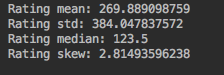
\includegraphics{stats}
		\end{figure}
		
		\begin{figure}[H]
			\caption{Rating Frequency}
			\label{fig:histogram_movie_ratings}
			\centering
			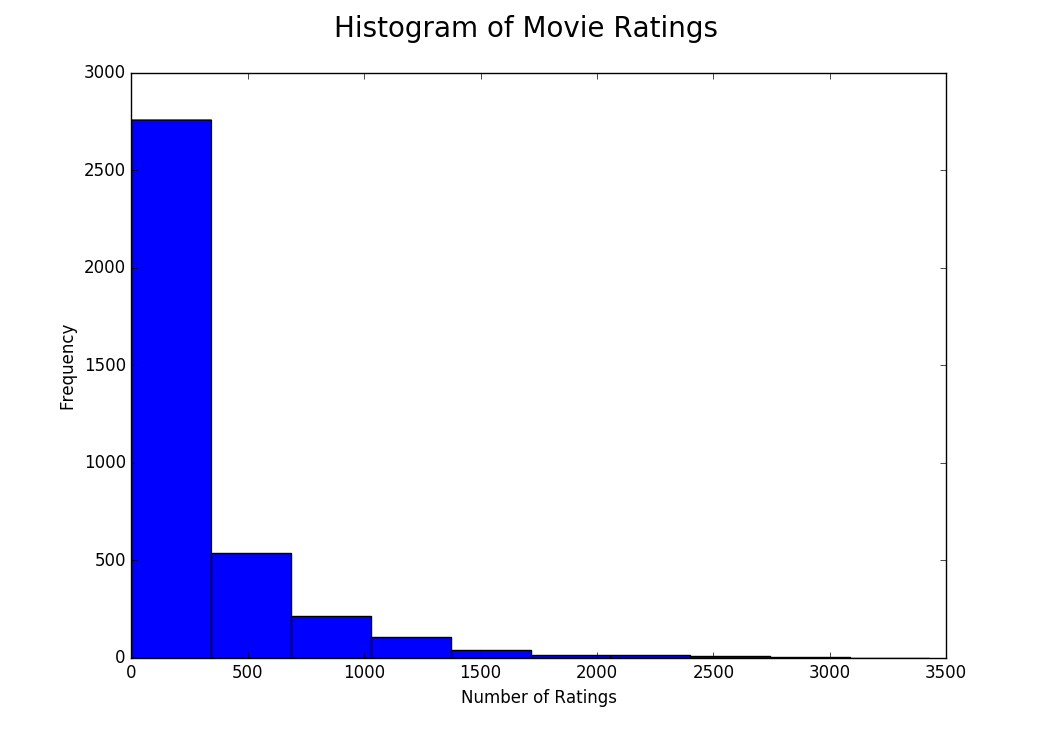
\includegraphics[height=6cm, width=10cm]{histogram_movie_ratings}
		\end{figure}
	\end{multicols}
	
	Figure \ref{fig:stats} and Figure \ref{fig:histogram_movie_ratings} shows that there is a positive skew in the distribution, i.e. the frequency of submitted ratings to each movie is bottom heavy. Because of this a top movie was defined as being a movie that has at least 300 ratings and the highest average rating. See the top 10 movies in \ref{fig:top_10_movies}.

	\begin{figure}[H]
		\caption{Top 10 Movies}
		\label{fig:top_10_movies}
		\centering
		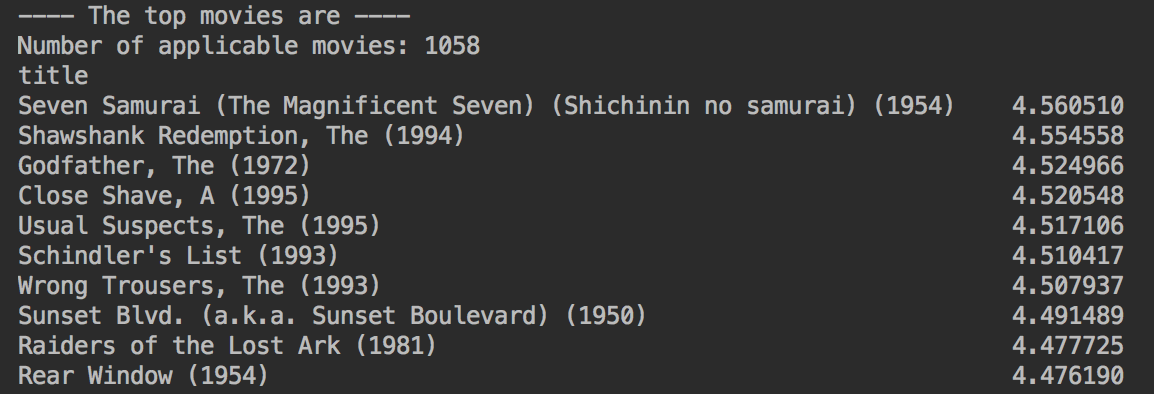
\includegraphics[height=7cm, width=17cm]{top_10_movies}
	\end{figure}
\end{enumerate}

\bibliographystyle{plain}
\bibliography{/Users/rasmusmunk/Documents/Bibtex/data_wrang.bib}

\end{document}